% !TeX program = xelatex
\documentclass[UTF8,a4paper,9.5pt,fontset=none]{ctexart}
\usepackage{iftex}
\ifXeTeX\else
  \PackageError{market-report}{This document must be compiled with XeLaTeX}
  {In Overleaf, open Menu -> Settings -> Compiler and select XeLaTeX.}
\fi
\setCJKmainfont{FandolSong-Regular}
\setCJKsansfont{FandolHei-Regular}
\setCJKmonofont{FandolFang-Regular}
\usepackage[left=1.55cm,right=1.55cm,top=1.45cm,bottom=1.50cm]{geometry}
\usepackage{amsmath,amssymb,booktabs,tabularx,array,multirow}
\usepackage{enumitem,hyperref,xcolor,float,microtype,graphicx,subcaption}
\hypersetup{colorlinks=true,linkcolor=black,citecolor=blue!55!black,urlcolor=blue!55!black}
\setlength{\parindent}{2em}
\setlength{\parskip}{0pt}
\setlist{nosep,leftmargin=1.8em}
\renewcommand{\baselinestretch}{0.98}
\newcolumntype{Y}{>{\raggedright\arraybackslash}X}
\pagestyle{plain}

\title{\vspace{-1cm}\textbf{基于金融新闻情绪与股票价格数据的市场趋势预测研究}}
\author{黄文轩\quad 王子轩\quad 林瀚羽\quad 彭琰轲\\深圳大学金融科技专业}
\date{}

\begin{document}
\maketitle
\vspace{-1.6em}
\begin{abstract}
本文研究每日金融与国际新闻情绪能否在历史量价信息之外提高道琼斯工业平均指数
（DJIA）下一交易日涨跌方向的预测能力。研究使用Combined News and DJIA公开数据，
涵盖2008年8月至2016年7月共1989个原始交易日和每日25条新闻标题。为避免同日新闻
与收盘价之间的时点歧义，本文不用原数据同日标签，而以$t$日新闻和量价特征预测
$t+1$日收益方向。VADER用于提取标题情绪，Logistic回归、随机森林与XGBoost用于
分类，并通过2014--2016年三个walk-forward测试窗口比较“仅量价”和“量价+新闻”。
结果显示，XGBoost加入新闻后平均ROC-AUC由0.472提升至0.504，但增量为0.035，
95\% bootstrap置信区间为$[-0.006,0.073]$，未达到统计显著。扣除10个基点仓位
调整成本后，新闻策略年化收益为$-13.1\%$，明显落后于同期DJIA买入持有。
研究说明新闻情绪可能提供微弱非线性信息，但该公开日频数据不足以支持稳定预测或
可交易结论。

\noindent\textbf{关键词：}金融新闻；情绪分析；VADER；股票趋势预测；XGBoost；
时间序列验证
\end{abstract}

\section{引言}
金融市场价格不仅受到历史交易行为影响，也会对新闻中的新增信息和投资者预期作出
反应。Tetlock发现媒体悲观语调与市场收益及成交量存在关系\cite{tetlock}；
Loughran和McDonald指出通用情绪词典在金融语境中可能产生误判\cite{lm}。
随着自然语言处理发展，新闻标题可以转化为连续情绪分数，再与结构化行情共同用于
趋势预测。

然而，相关研究容易因数据时点处理不当而高估效果。若使用当天全部新闻解释当天
收盘涨跌，部分新闻可能在收盘后才发布；若随机打乱时间序列，未来市场状态也会进入
训练集。因此本文采用更严格的下一交易日任务：使用$t$日新闻和截至$t$日可计算的
量价指标预测$t+1$日DJIA方向，并用时间递增窗口评价样本外表现。

本文回答三个问题：新闻情绪能否提高方向预测AUC；提升是否具有统计显著性；模型
信号在交易成本后是否具有经济价值。研究同时报告弱结果和失败结果，不以单一年份
或单一指标支持结论。

\section{相关研究}
\subsection{新闻情绪与市场反应}
Tetlock的经典研究表明媒体悲观程度包含与市场活动相关的信息\cite{tetlock}。
Loughran--McDonald金融词典说明金融文本需要领域处理\cite{lm}。
VADER结合情绪词典、程度副词、否定和标点规则，能够输出$[-1,1]$范围的compound
分数，具有透明、轻量和可复现的优点\cite{vader}。其不足是未专门在金融语料训练，
因此本文将其视为课程实验基线，而非最优情绪模型。

\subsection{预测模型与验证}
Logistic回归适合构建线性可解释基线；随机森林通过多树集成捕捉非线性\cite{rf}；
XGBoost使用梯度提升和正则化，适合中小规模表格数据\cite{xgboost}。金融时间序列
必须按时间切分，并应在滚动特征窗口与测试期之间设置隔离，避免信息泄漏
\cite{lop}。本文据此设置三年滚动测试和20个交易日隔离期。

\section{数据与变量}
\subsection{数据来源}
数据来自Kaggle的Daily News for Stock Market Prediction公开项目及其GitHub镜像
\cite{dataset}。新闻表包含\texttt{Date}、原同日\texttt{Label}以及
\texttt{Top1--Top25}标题；行情表包含DJIA开盘价、最高价、最低价、收盘价、成交量
和复权收盘价。原始新闻表有1989日。合并行情并删除20日滚动窗口不足和最后一个
无下一日收益的样本后，得到1968个交易日、49193条有效标题，时间为
2008年9月8日至2016年6月30日。下一日上涨样本占53.51\%。

\subsection{情绪与价格特征}
清洗标题中的字节串标记、引号、HTML实体和多余空白。对每日标题$j$计算VADER
compound分数$s_{j,t}$，并构造日均情绪：
\begin{equation}
\bar{s}_t=\frac{1}{N_t}\sum_{j=1}^{N_t}s_{j,t}.
\end{equation}
同时计算情绪标准差、最大值、最小值、正向占比、负向占比、中性占比、一阶滞后及
情绪变化。实际样本中，下一日上涨组的日均情绪为$-0.2150$，下跌组为$-0.2168$，
两组均值差异极小。

价格特征包括1/5/10/20日收益率、5/20日均线差、5日和20日波动率、成交量变化率、
日内振幅与5日动量方向。目标变量为：
\begin{equation}
y_{t+1}=\mathbb{I}\left(P_{t+1}/P_t-1>0\right).
\end{equation}
原数据自带同日标签不参与主实验，从而保证特征先于预测目标。

\begin{figure}[H]
\centering
\begin{subfigure}[t]{0.48\textwidth}
  \centering
  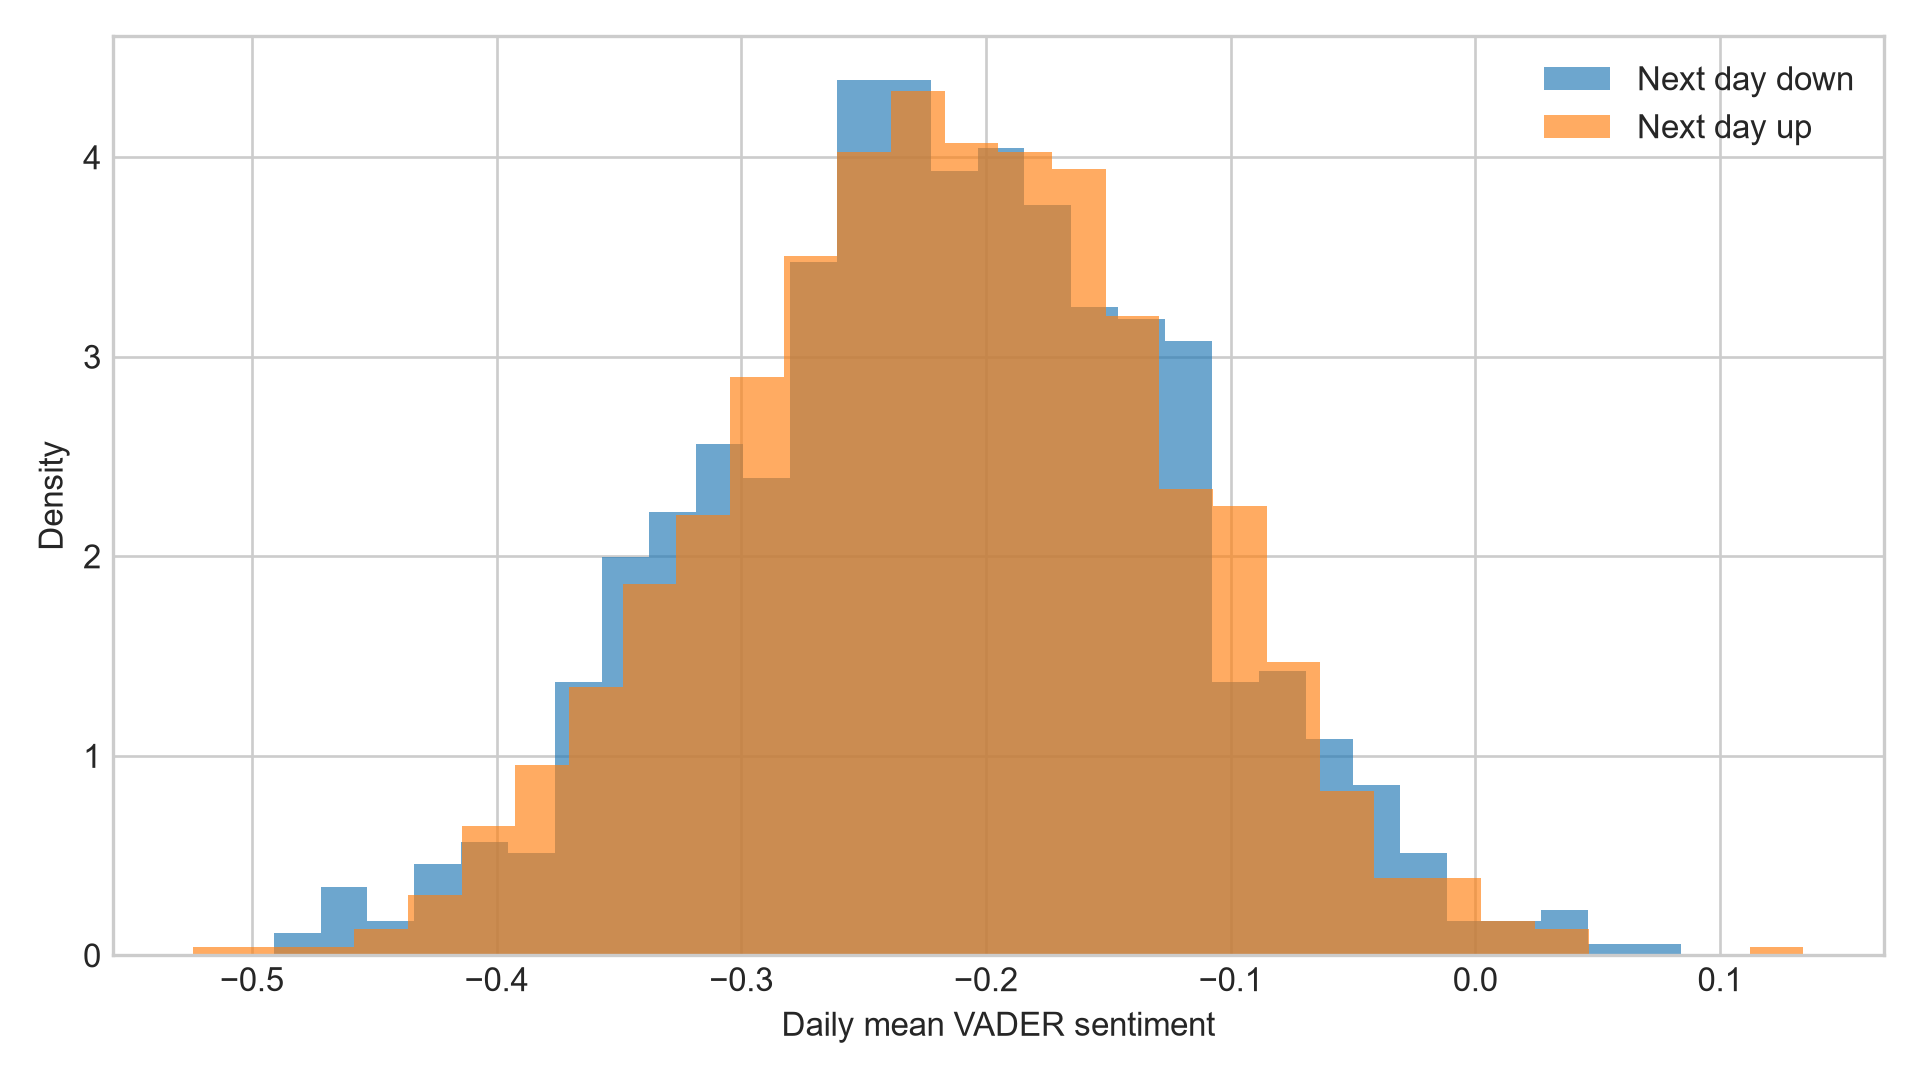
\includegraphics[width=\linewidth]{figures/sentiment_distribution.png}
  \caption{上涨日与下跌日之前的情绪分布}
\end{subfigure}
\hfill
\begin{subfigure}[t]{0.48\textwidth}
  \centering
  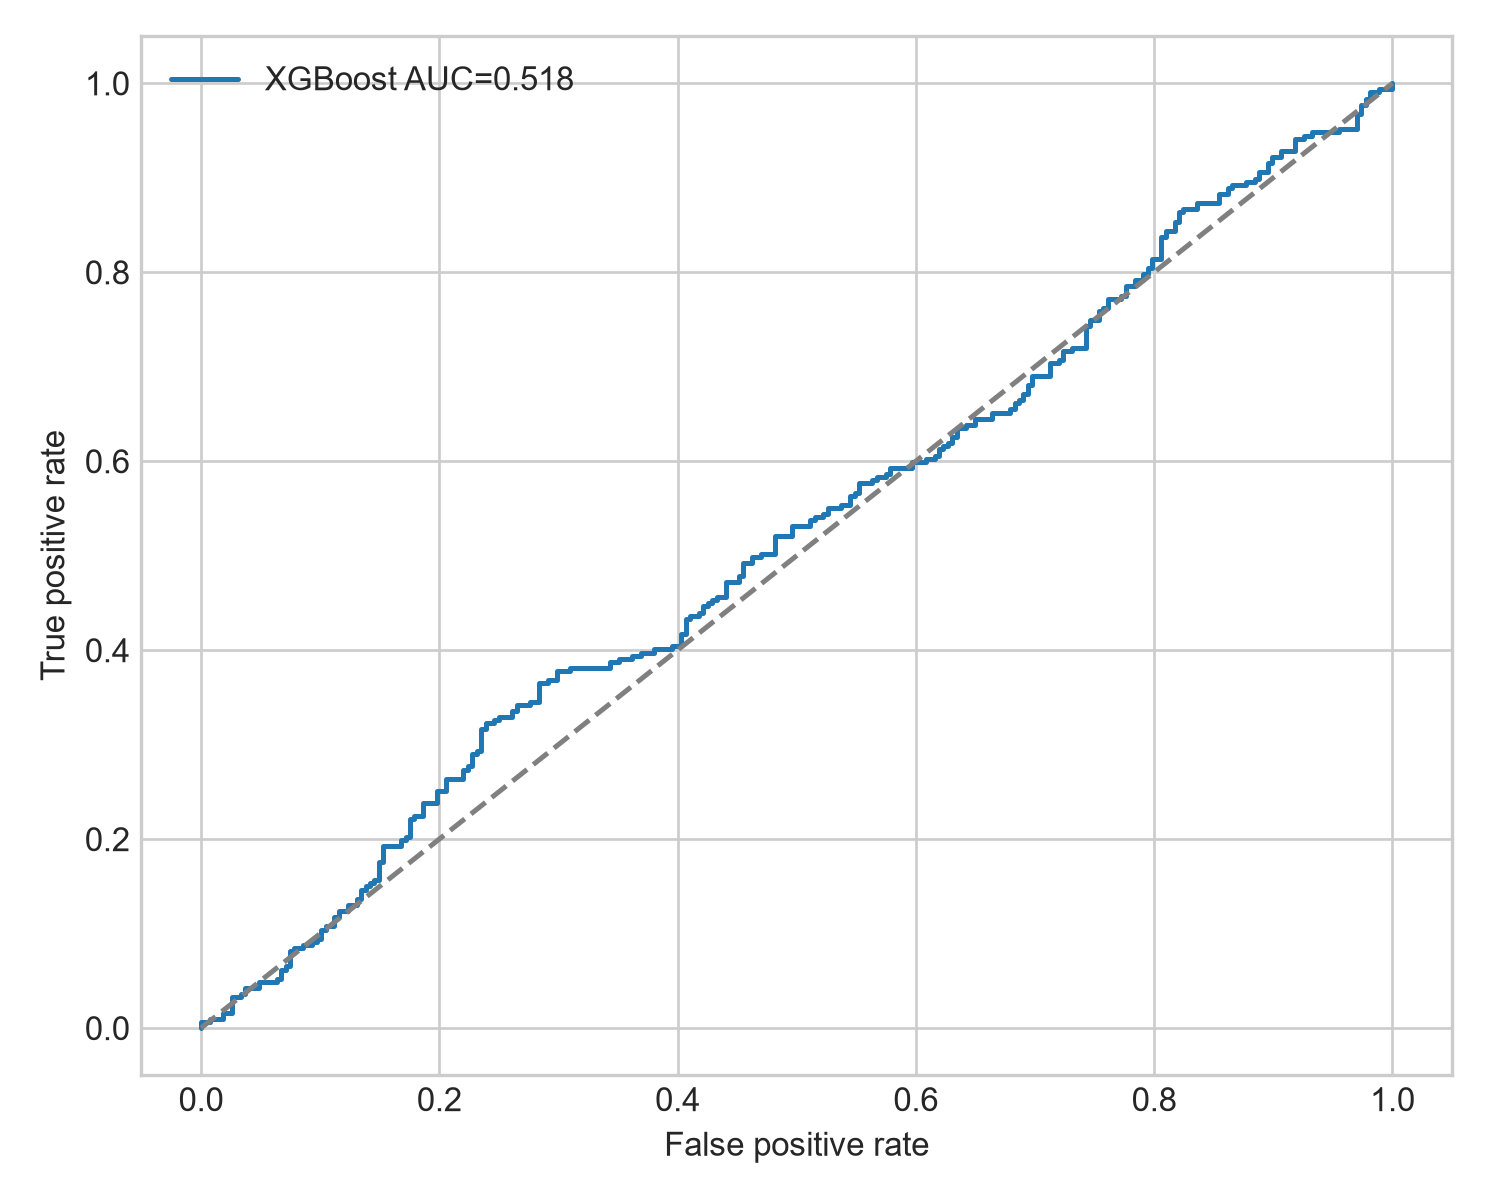
\includegraphics[width=\linewidth]{figures/xgboost_roc_curve.png}
  \caption{XGBoost量价加新闻的合并ROC曲线}
\end{subfigure}
\caption{新闻情绪分布与样本外识别能力}
\label{fig:sentiment-roc}
\end{figure}

\section{研究方法}
\subsection{模型与消融设计}
本文训练Logistic回归、随机森林和XGBoost。设置P组与P+N组：P组仅含量价技术
指标；P+N组增加新闻情绪变量。同一算法两组结果之差用于衡量新闻的增量价值。
Logistic使用类别权重和平滑标准化；随机森林包含500棵树并限制深度与叶节点样本；
XGBoost使用350棵浅树、0.025学习率、行列采样和$L_1/L_2$正则化。

\subsection{walk-forward验证}
测试期为2014、2015和2016年。每一折以测试年前一年作为验证期、更早数据作为训练期，
并在验证和测试开始前设置20个交易日隔离。例如2014测试折使用2012年及以前训练、
2013年验证、2014年测试。分类阈值在验证集上按最大F1确定，再固定应用于测试集。
缺失值填补和标准化只在训练集拟合。

\subsection{指标、显著性与回测}
报告ROC-AUC、PR-AUC、F1、平衡准确率和Brier分数。由于样本中上涨比例为53.51\%，
F1可能因偏向预测上涨而较高，因此以AUC和平衡准确率作为主要判断依据。对XGBoost
两组预测进行2000次配对bootstrap，计算AUC增量的95\%置信区间。

经济性检验在P+N模型预测上涨概率不低于0.55时持有DJIA，否则持有现金。仓位每次
变化扣除10个基点成本，报告年化收益、波动率、夏普比率和最大回撤。

\section{实验结果}
\subsection{模型预测结果}
\begin{table}[H]
\centering\small
\caption{2014--2016年测试窗口平均结果}
\begin{tabular}{llccccc}
\toprule
模型 & 特征 & AUC & PR-AUC & F1 & 平衡准确率 & Brier\\
\midrule
Logistic & P & 0.493 & 0.533 & 0.699 & 0.500 & 0.251\\
Logistic & P+N & 0.489 & 0.551 & 0.692 & 0.498 & 0.252\\
随机森林 & P & 0.471 & 0.561 & 0.699 & 0.503 & 0.253\\
随机森林 & P+N & 0.485 & 0.540 & 0.694 & 0.494 & 0.251\\
XGBoost & P & 0.472 & 0.551 & 0.680 & 0.489 & 0.263\\
XGBoost & P+N & \textbf{0.504} & 0.555 & 0.695 & 0.501 & 0.256\\
\bottomrule
\end{tabular}
\label{tab:model-results}
\end{table}

表\ref{tab:model-results}显示，所有模型的AUC均接近0.5，说明下一日方向预测困难。
Logistic加入新闻后AUC略降0.004；随机森林提高0.014；XGBoost提高0.032。
这表明新闻变量可能只通过非线性交互提供少量信息。XGBoost P+N在三个测试年的
AUC分别为0.519、0.533和0.462，跨年份并不稳定。

\begin{figure}[H]
\centering
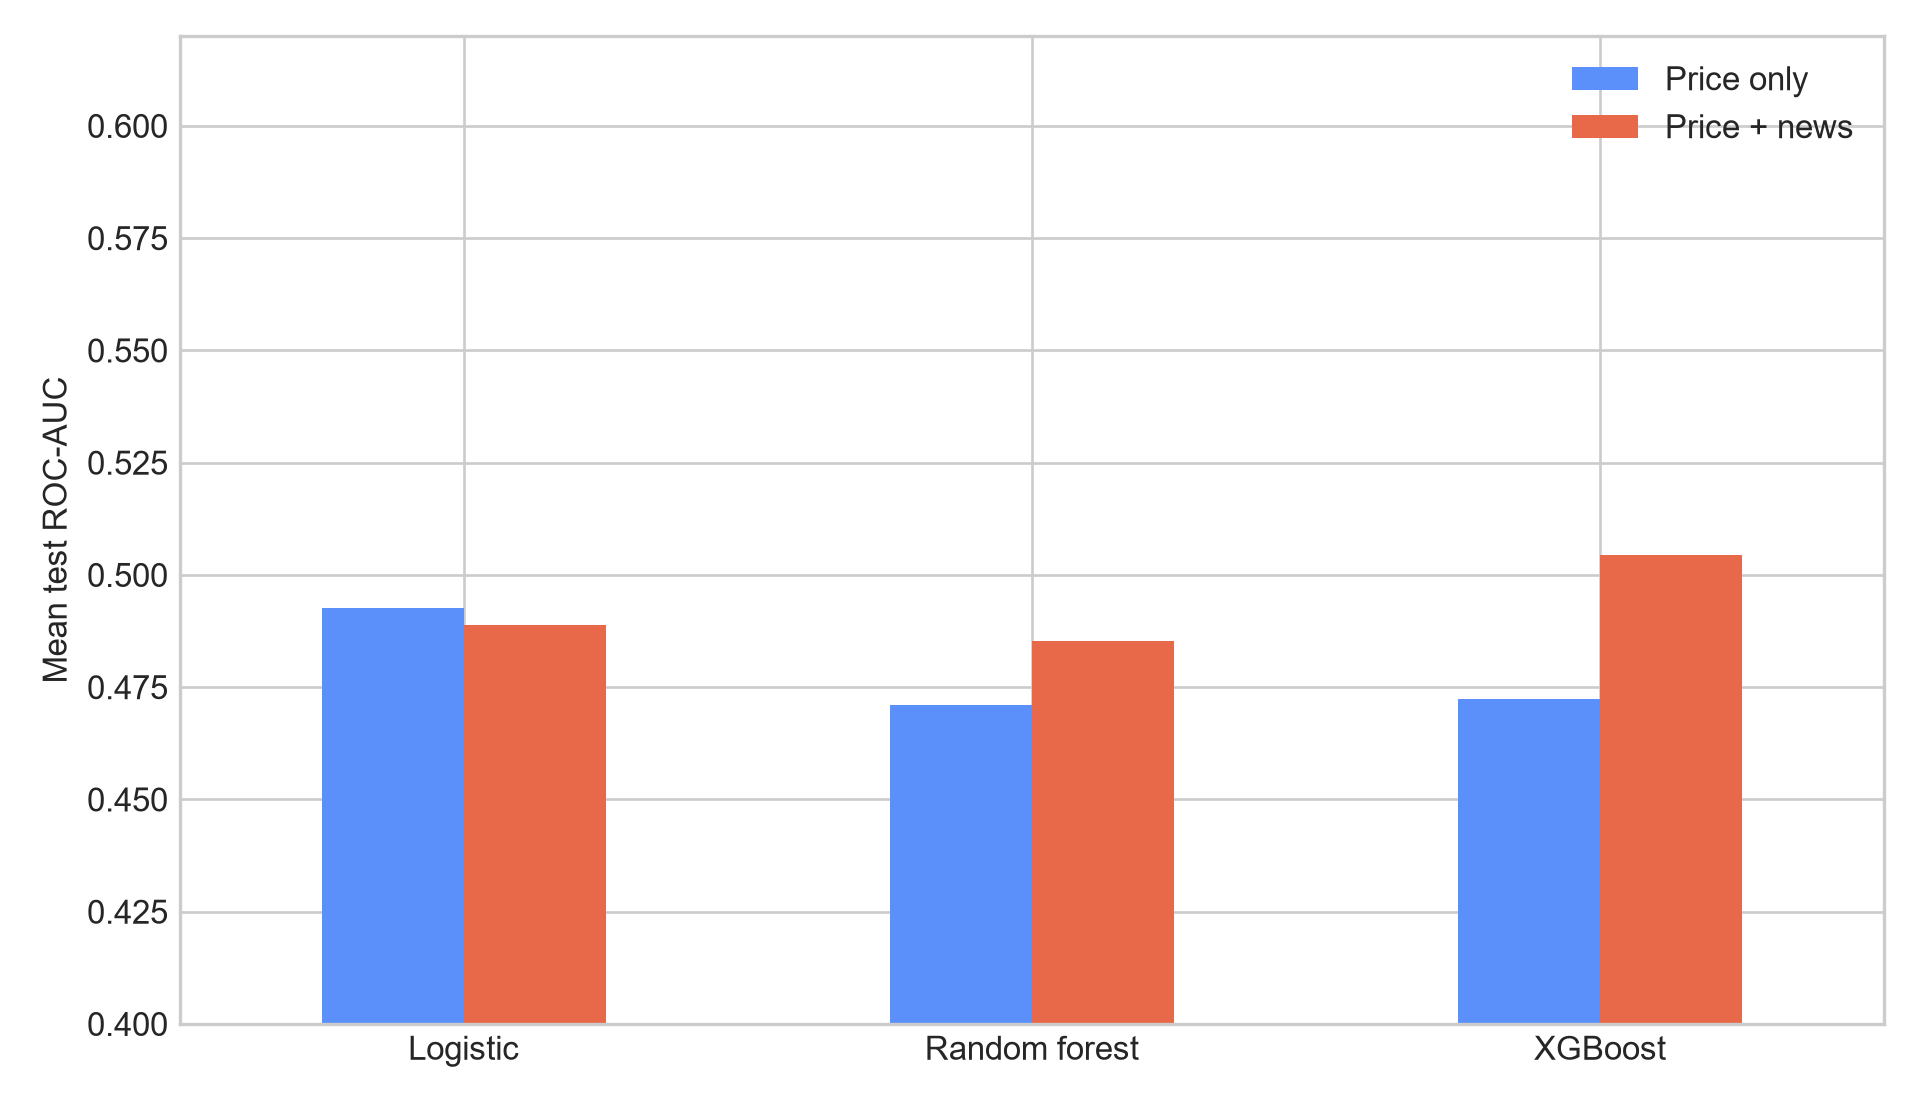
\includegraphics[width=0.72\textwidth]{figures/model_auc_comparison.png}
\caption{三类模型加入新闻前后的平均测试AUC}
\label{fig:auc}
\end{figure}

将2014--2016年XGBoost配对预测合并后，新闻带来的AUC增量为0.0348。
2000次bootstrap的95\%置信区间为$[-0.0060,0.0734]$，包含0，因此不能拒绝
“新闻没有增量效果”的原假设。图\ref{fig:sentiment-roc}中上涨和下跌组情绪分布
高度重合，也与这一结论一致。

\subsection{经济意义}
以0.55为持仓阈值时，策略在575个样本外交易日中有48.52\%时间持仓。扣除10bp
仓位调整成本后，策略年化收益为$-13.12\%$，年化波动率8.69\%，夏普比率$-1.51$，
最大回撤$-29.46\%$；同期DJIA买入持有年化收益约8.95\%。图\ref{fig:return}
显示策略持续落后于市场，因此统计上微弱的AUC提升没有转化为经济价值。

\begin{figure}[H]
\centering
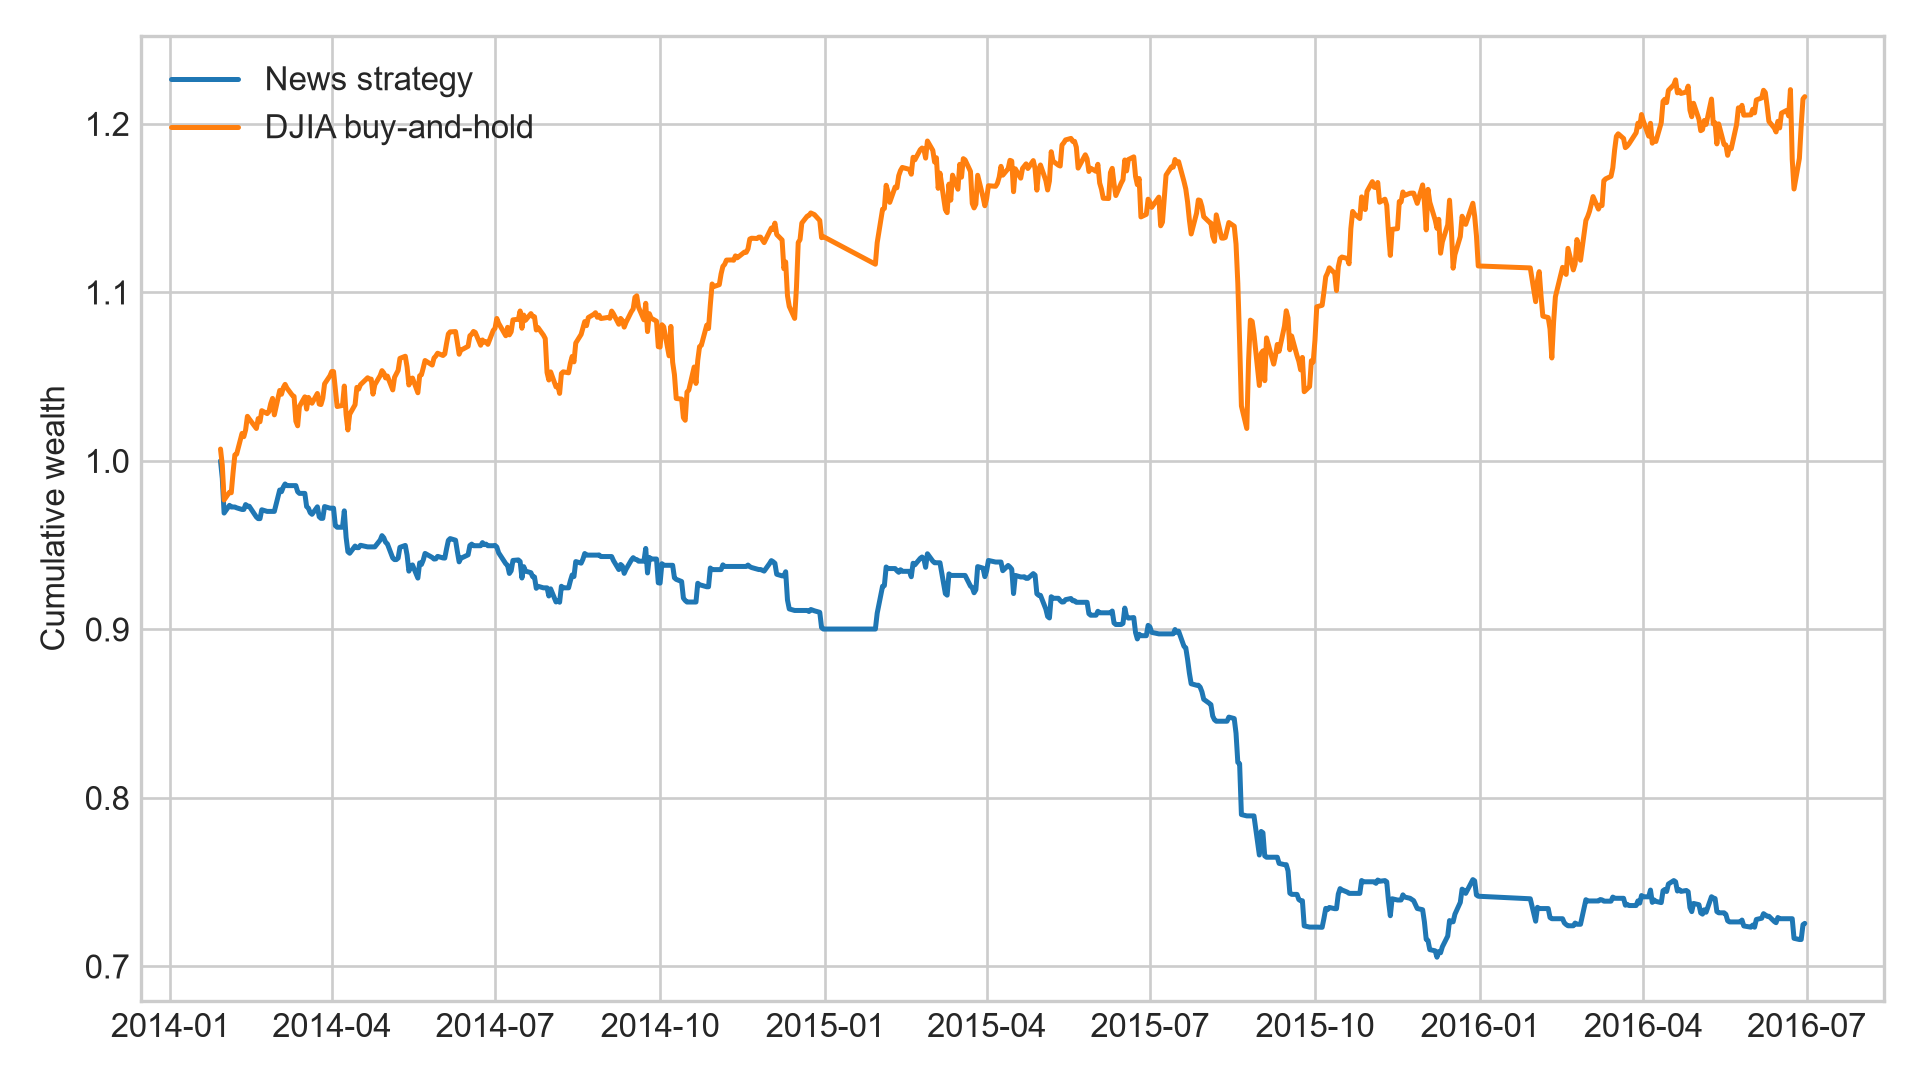
\includegraphics[width=0.78\textwidth]{figures/cumulative_returns.png}
\caption{XGBoost新闻策略与DJIA买入持有的样本外累计净值}
\label{fig:return}
\end{figure}

\section{讨论、局限与稳健性}
结果不支持“新闻情绪能够稳定预测下一交易日方向”的强结论。可能原因包括：
第一，每日热点新闻以国际政治和社会事件为主，不全是直接影响DJIA公司的金融新闻；
第二，VADER并非金融领域模型，无法充分理解金融术语与事件语义；第三，25条标题
被压缩为少量日统计量，可能丢失事件主体和重要性；第四，日频市场对公开新闻的吸收
速度较快；第五，样本仅约2000日，且2016年测试期只到6月底。

本研究也存在限制。数据没有逐条精确发布时间，无法区分盘前、盘中和盘后新闻；
回测使用指数收益且未加入滑点；模型超参数采用固定的保守设置；VADER结果未与
FinBERT比较。后续稳健性检验可包括：使用FinBERT替代VADER；以TF-IDF文本特征
建立新闻模型；分别研究盘前新闻；延长到更新年份；预测收益超过交易成本阈值而非
简单涨跌；使用概率校准和不同持仓阈值。

\section{结论}
本文基于1968个交易日和49193条新闻标题，构建了新闻情绪与DJIA量价融合的下一日
趋势预测实验。严格的walk-forward结果显示，XGBoost加入新闻后平均AUC从0.472
提高到0.504，但bootstrap置信区间包含0，且回测显著亏损。由此可见，该数据和
VADER聚合情绪最多提供微弱、不稳定的非线性信号，不足以支持稳定预测或交易应用。
这一负结果说明，金融机器学习研究中严格时间对齐、样本外验证和经济检验比单纯提高
模型复杂度更重要。

\begin{thebibliography}{99}\small
\bibitem{tetlock} Tetlock, P. C. Giving Content to Investor Sentiment: The Role of Media in the Stock Market. \emph{The Journal of Finance}, 62(3):1139--1168, 2007.
\bibitem{lm} Loughran, T., McDonald, B. When Is a Liability Not a Liability? \emph{The Journal of Finance}, 66(1):35--65, 2011.
\bibitem{vader} Hutto, C. J., Gilbert, E. VADER: A Parsimonious Rule-based Model for Sentiment Analysis of Social Media Text. \emph{ICWSM}, 2014.
\bibitem{rf} Breiman, L. Random Forests. \emph{Machine Learning}, 45:5--32, 2001.
\bibitem{xgboost} Chen, T., Guestrin, C. XGBoost: A Scalable Tree Boosting System. \emph{KDD}, 785--794, 2016.
\bibitem{lop} L\'opez de Prado, M. \emph{Advances in Financial Machine Learning}. Wiley, 2018.
\bibitem{dataset} Sun, J. Daily News for Stock Market Prediction, Version 1. Kaggle, 2016. \url{https://www.kaggle.com/datasets/aaron7sun/stocknews}.
\end{thebibliography}
\end{document}
